\documentclass[french]{beamer}
\usetheme{default}

\usepackage[T1]{fontenc}
\usepackage[utf8]{inputenc}
\usepackage{lmodern}
\usepackage{geometry}
\usepackage{babel}
\usepackage{graphicx}
\graphicspath{ {./images/} }

\usepackage{listings}

\usepackage{standalone}

\usepackage{tikz}
\usetikzlibrary{calc,trees,positioning,arrows,chains,shapes.geometric,%
	decorations.pathreplacing,decorations.pathmorphing,shapes,%
	matrix,shapes.symbols,fit,arrows.meta,backgrounds}


\lstset{ %
	texcl=true,
	escapeinside={//}{\^^M},
}

\title{Étude de quelques algorithmes de joueurs artificiels participants à des jeux de stratégie en temps réel}
\author{Dimitri \bsc{Cocheril-Crèvecœur} \\ 13960}
\begin{document}
\begin{frame}[plain]
    \maketitle
\end{frame}
\begin{frame}{Plan}
	\begin{enumerate}
		\item Présentation du problème
		\item Moteur
		\item Stratégies testées
	\end{enumerate}
\end{frame}
\begin{frame}{StarCraft}
	\begin{figure}
		\centering
		\begin{minipage}{0.5\textwidth}
			Jeu de stratégie en temps réel:
			\begin{itemize}
				\item Jeux simultané
				\item Deux joueurs s'affrontent pour le contrôle d'une carte
				\item Gestion de ressources : minage, création d'unitées, de bases (stratégie)
				\item Combat entre unitées (tactique)
			\end{itemize}
		\end{minipage}\hfill
		\begin{minipage}{0.5\textwidth}
			\centering
			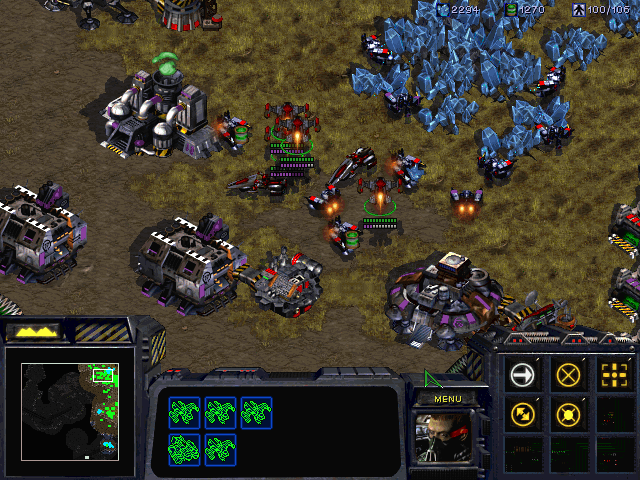
\includegraphics[width=0.99\textwidth]{screen_starcraft.png}
		\end{minipage}
	\end{figure}
\end{frame}
\begin{frame}{Modèles existants}
	\begin{itemize}
		\item IA de Google : \textit{AlphaStar} 
			\\Apprentissage supervisé puis par renforcement
		\item Robots ("bots") :
	\end{itemize}
	\centering
	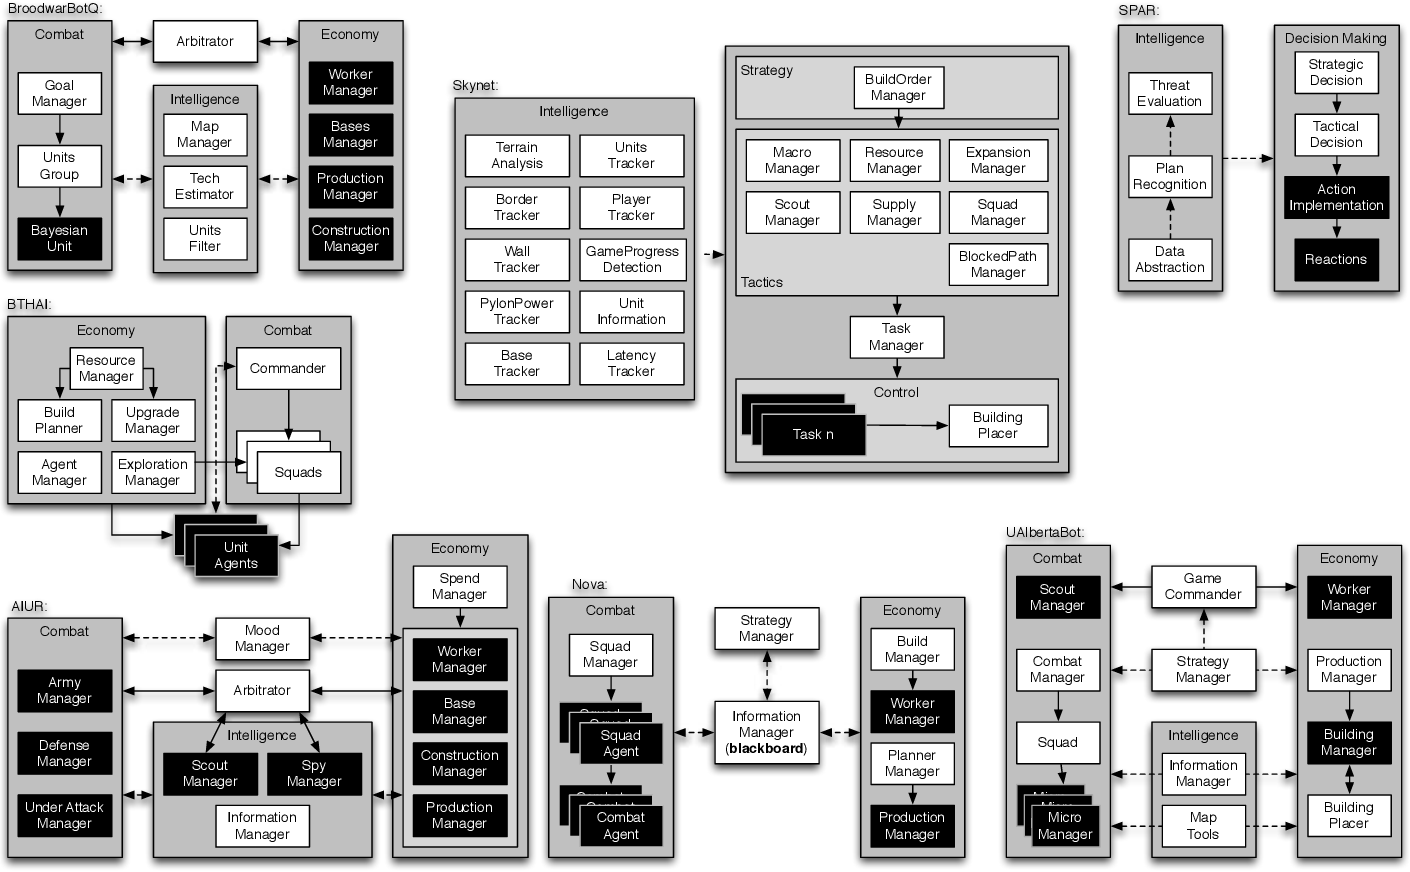
\includegraphics[width=0.7\textwidth]{architectures.png} 
\end{frame}
\begin{frame}{StarCraft}
\begin{figure}
	\centering
	\begin{minipage}{0.45\textwidth}
		On se concentre ici sur la partie "combat" :

		Deux joueurs disposent d'unitées pouvant bouger et attaquer celles adverses

		Chaque joueur doit tuer toute les unitées ennemies
	\end{minipage}\hfill
	\begin{minipage}{0.5\textwidth}
		\centering
		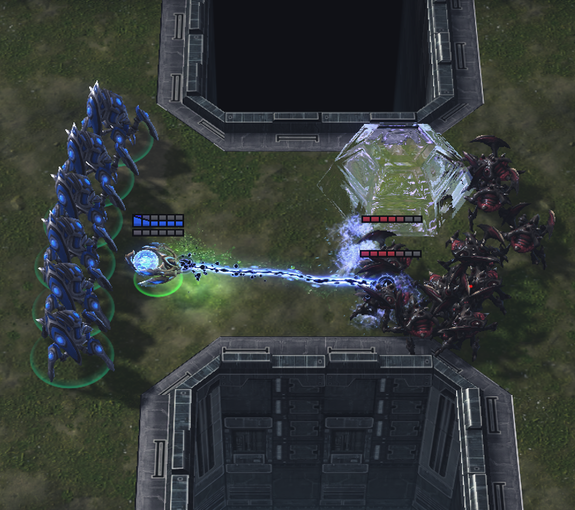
\includegraphics[width=0.99\textwidth]{screen_starcraft_combat.png}
	\end{minipage}
\end{figure}
\end{frame}
\begin{frame}{Problème}
	\begin{enumerate}
		\item Facteur de branchement entre $10^{50}$ et $10^{200}$
		\item Durée typique d'une partie : $25$ minutes donc $25\times60\times24=36000$ états
	\end{enumerate}
\end{frame}
\begin{frame}{Développement moteur du jeu}
	\begin{figure}
		\centering
		\begin{minipage}{0.49\textwidth}
			\centering
			\includestandalone[width=\linewidth]{images/tikz_moteur}
		\end{minipage}\hfill
		\begin{minipage}{0.49\textwidth}
			\centering
			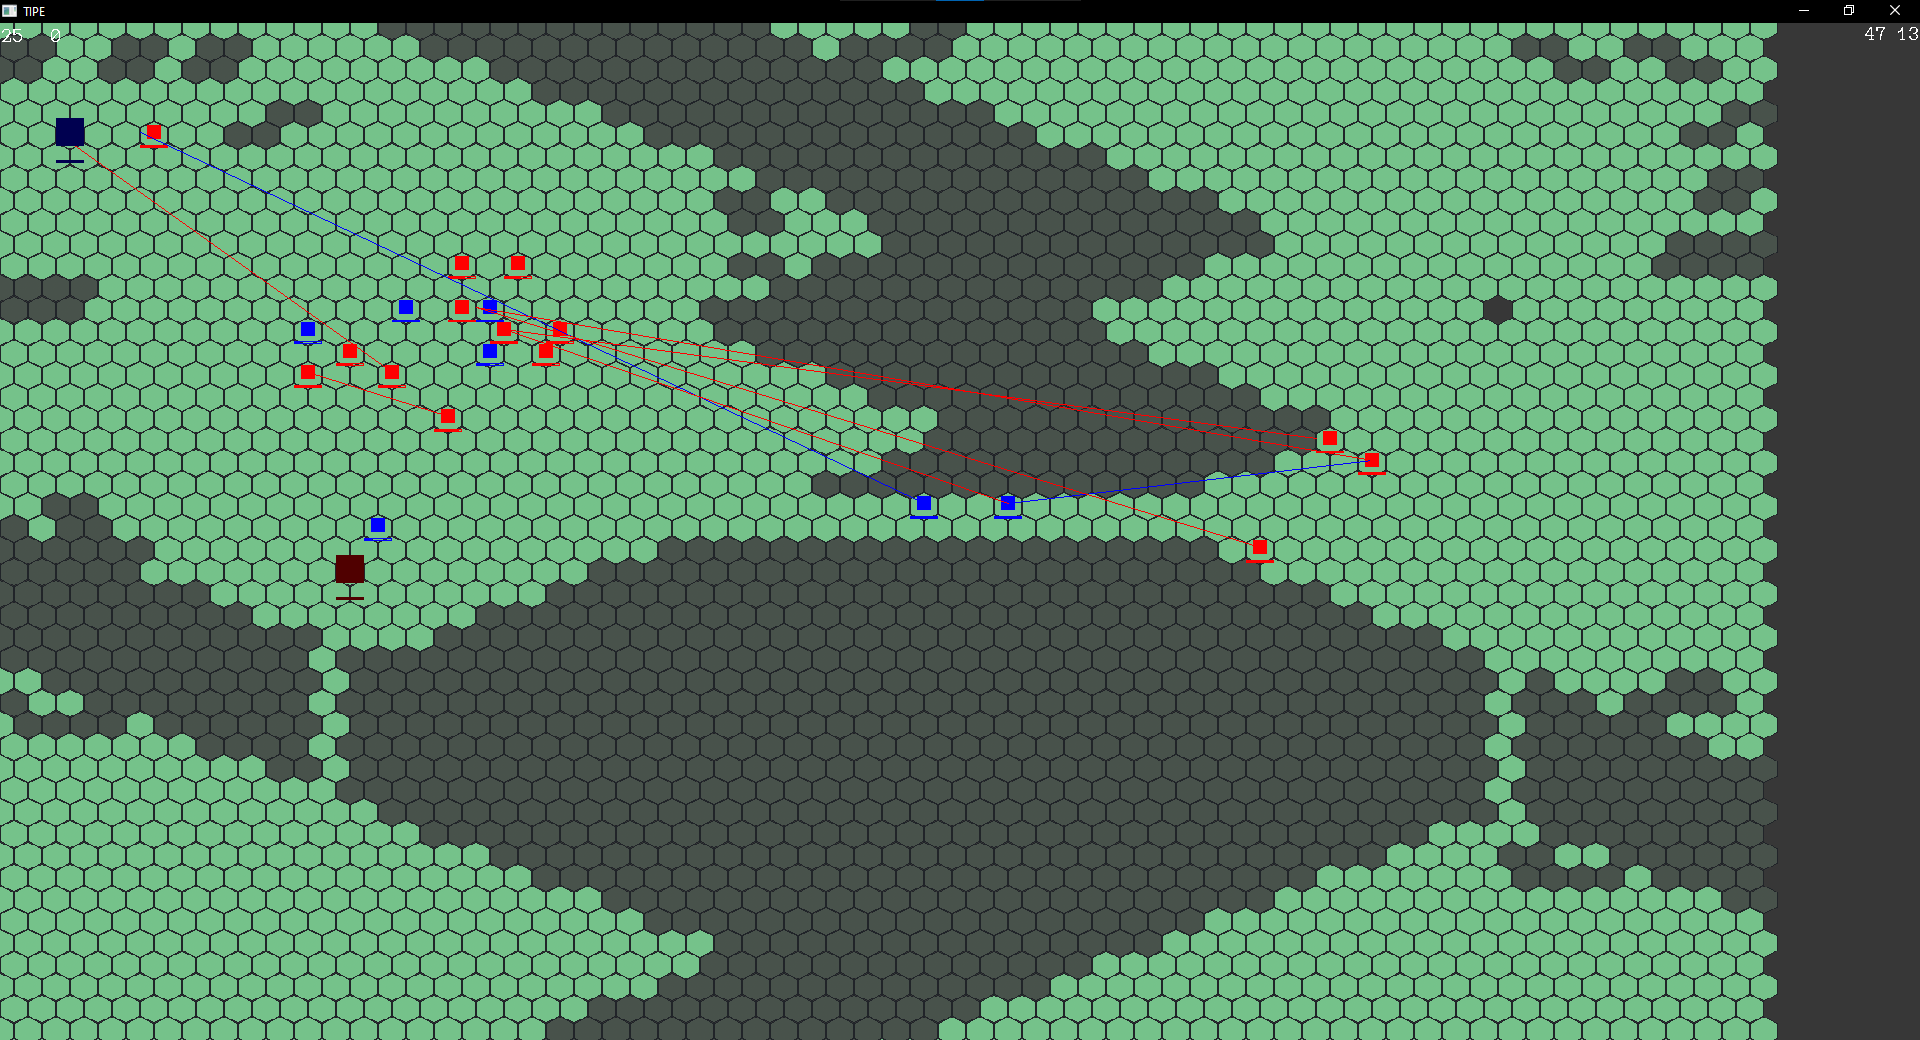
\includegraphics[width=0.95\textwidth]{screen_carte_pleine.png}
		\end{minipage}
	\end{figure}
\end{frame}
\begin{frame}[fragile]
	\small
	\begin{lstlisting}[language=C++,basicstyle=\ttfamily,keywordstyle=\color{red}]
void game_class::play() const
{
    for (const auto p : players_)
    /*Pour chaque joueur...*/
    {
        p->moves_get(this, state_);
        /*..on choisit les actions..*/
    }
    state_->moves_make(map_);
    /*..et on effectue les actions.*/
}
	\end{lstlisting}
\end{frame}
\begin{frame}[fragile]
\small
\begin{lstlisting}[language=C++,basicstyle=\ttfamily,keywordstyle=\color{red}]
	void game_class::play() const
	{
		for (const auto p : players_)
		/*Pour chaque joueur...*/
		{
			p->moves_get(this, state_);
			/*..on choisit les actions..*/
		}
		state_->moves_make(map_);
		/*..et on effectue les actions.*/
	}

\end{lstlisting}
\end{frame}
\begin{frame}{Problème de la recherche de chemin}
	\begin{itemize}
		\item Optimisation compliquée :
		
		On utilise un A* pondérée à 5 (trouvé de manière expérimentale)
		
		\item Parrallélisation du programme
		
		On alloue les espaces dynamiquements au lieu d'utiliser le tas pour éviter la conccurence
	\end{itemize}
Parrallélisation :
\end{frame}
\begin{frame}{Joueur aléatoire}
	Joueur témoin : choisis une action aléatoire, et l'effectue avant d'en choisir une autre aléatoirement
	\vspace*{1em}
	
	On effectue 10000 combats sur une carte vide entre deux joueurs aléatoires avec 50 unités chacun:
	\vspace*{1em}
	
	Victoires de joueur 0 : 4689
	
	Victoires de joueur 1 : 5306
	
	Égalités : 5
\end{frame}
\begin{frame}{Stratégie naïve : attaque par puissance}
	Toutes nos unités attaquent l'unitée ennemie avec la plus grande puissance
	
	Résultats contre joueur aléatoire avec 50 unités:
	
	100\% de victoire pour joueur aléatoire
\end{frame}
%\begin{frame}{Stratégie naïve : attaquer par distance}
	
%\end{frame}
\begin{frame}{Utilisation MCTS}
 
\end{frame}
\begin{frame}{Rassemblement des unitées : DBSCAN}
	
\end{frame}
\end{document}
